%% poster.tex
%% Vorlage fr A0-Poster
%% Harry Schmidt
%% 25.04.2003

%% translation instructions (there should be a better way):
%% latex ...
%% dvips -Ppdf -D9600 ...
%% psresize -w84cm -h118.8cm ... outfile.ps
%% edit postscript to position and size poster correctly
%%    bounding box in ps: 0 0 2380 3368
%%    after %%EndComments add:  gsave 0 -140 translate
%%    before showpage     add:  grestore
%% (adjust voffset and hoffset below to center text on page)
%% ps2pdf -sPAPERSIZE=a0 poster2a.ps


\documentclass{theo1poster}[2003/04/25]
\textwidth=12.5in                 % real width of latex text 
\textheight=9in                % height of latex text
\special{papersize=13in,10.5in}   % small width ensures portrait orientation
\addtolength{\voffset}{-.7in}
\addtolength{\textheight}{1.5cm}
\addtolength{\voffset}{52pt}  %% depends on actual length of poster
\addtolength{\hoffset}{0pt}   %% probably universal
%\usepackage[american,ngerman]{babel}
\usepackage[latin1]{inputenc}
\usepackage[T1]{fontenc}
%\usepackage{ae}
\usepackage{amsmath,amssymb,psfrag,pifont}
\usepackage{graphicx}

\input defs
%% Farben

\definecolor{lightblue}{rgb}{0.75,0.8,1}
\definecolor{graublau}{rgb}{0.85,0.85,0.9}
\definecolor{gruen}{rgb}{0.0,0.4,0.0}
\definecolor{alexblue}{rgb}{0.8,0.64,0.0}
\definecolor{strangeyellow}{rgb}{0.875,1.0,0.08}
\definecolor{verylightgray}{gray}{0.99}
\definecolor{meinrot}{rgb}{0.8,0.1,0.2}
\definecolor{lightocker}{rgb}{1,0.9,0.6}
\definecolor{orange}{rgb}{1,0.5,0}
\definecolor{darkorange}{rgb}{0.7,0.35,0}


\definecolor{sheetbg}{rgb}{0.75,0.8,1}
\definecolor{boxbg}{rgb}{1,1,0.95}
\definecolor{boxrahmen}{rgb}{0.11,0.15,0.4}


%% Stil-Befehle fr das Poster, kann fr jedes
%% einzelne Poster festgelegt werden

\posterbgcolor{white}    %% Hintergrundfarbe des Posters
%\posterbgcolor{lightocker}
%\posterbgcolor{lightblue}
%\posterbgcolor{graublau}


%\titlecolor{black}         %% Farbe des Titels
\headingcolor{black}       %% Farbe der �erschriften
%\headingcolor{meinrot}

%\headingfont{\sffamily}    %% Font der �erschriften
%\headingfontsize{\large}   %% Fontgr�e der �erschriften

\sheetframewidth{1mm}    %% Breite des Sheet-Rahmens
\sheetframesep{3pt}        %% Abstand des Textes vom Rahmen

\sheetframecolor{boxrahmen}    %% Farbe des Sheet-Rahmens
%\sheetframecolor{boxbg}
\sheetbgcolor{white}       %% Farbe des Sheet-Hintergrunds
%\sheetbgcolor{verylightgray}

\colorsheets               %% Wird automatisch von \sheet..color  ausgefhrt
%\nocolorsheets             %% Default, solange \sheet..color nicht aufgerufen
%\roundsheets               %% Abgerundete Ecken ohne Farbe
\roundcolorsheets          %% Farbig und abgerundete Ecken

%\highlightcolor{lightocker} %% Farbe fr Hervorhebungen (Formeln)

%\renewcommand*\sectfont{\sffamily}
%\renewcommand*\sectfont{\bfseries\mathversion{bold}}

%\renewcommand*\bfdefault{b}


%% Sonstige Befehle

\renewcommand{\labelitemi}{\ding{228}}
\renewenvironment{itemize}% Liste mit bullet in gegebenem Abstand
                              % von linkem Rand der umschliessenden Umgebung
                              % M. Stollsteimer, 15.1.2001
 {\begin{list}{\labelitemi}%
       {%
%        \setlength{\topsep}{0pt}% Abstand vor Liste
        \setlength{\leftmargin}{0pt}% Raum vor bullet
        \setlength{\itemindent}{0pt}% Einrckung der ersten Zeile
        \settowidth{\labelwidth}{\labelitemi}%
        \addtolength{\labelsep}{\itemindent}
        \addtolength{\leftmargin}{\labelwidth}%
        \addtolength{\leftmargin}{\labelsep}%
        \addtolength{\leftmargin}{-\itemindent}%
       }%
 }
 {\end{list}}

\newenvironment{itemizenotopsep}{% Wie oben, nur mit \topsep=0pt
  \begin{list}{\labelitemi}%
    {%
      \setlength{\topsep}{0pt}% Abstand vor Liste
      \setlength{\leftmargin}{0pt}% Raum vor bullet
      \setlength{\itemindent}{0pt}% Einrckung der ersten Zeile
      \setlength{\itemsep}{0.5pt}% vertikaler Abstand von Items
      \setlength{\parsep}{1.5pt}%
      \settowidth{\labelwidth}{\labelitemi}%
      \addtolength{\labelsep}{\itemindent}
      \addtolength{\leftmargin}{\labelwidth}%
      \addtolength{\leftmargin}{\labelsep}%
      \addtolength{\leftmargin}{-\itemindent}}%
    }
  {\end{list}}


%% Daten fr den Titel

\title{Towards continuous symmetry reduction\\ 
for high dimensional flows
}

\author{\textbf{Evangelos Siminos}\ensuremath{^\diamond} and Predrag Cvitanovi\'c}
\newlength{\addresswidth}
 
\address{
	\begin{minipage}[c]{\textwidth}
		\begin{center}
			Center for Nonlinear Science, School of Physics,\\
			Georgia Institute of Technology, Atlanta, GA 30332-0430\\
			\ensuremath{\diamond} siminos@gatech.edu
	 	 \end{center}
         \end{minipage}
}



%% Wem die Titelei nicht gef�lt:
%\renewcommand{\maketitle}{eigene Titelei}




\begin{document}


\begin{poster}{4}


\begin{sheet}{Continuous symmetry in PDE's}


\begin{itemize}
 \item Continuous symmetry arizes in many PDE's and their truncations, e.g.
	\begin{itemize}
		\item \KSe~in periodic domain ($O(2)$)
		\item \PCf~($O(2)\times O(2)$)
		\item Maxwell-Bloch equations for a detuned ring laser ($SO(2)$)
	\end{itemize}
 \item For any solution a continuum of ``rotated'' solutions exists
 \item Phase space structure ``blurred'' - recurrence up to symmetry
 \item \Poincare~sections hard to construct 
\end{itemize}

\end{sheet}




\begin{sheet}{\CLe}
 
 \begin{itemize}
 \item Drastic truncation of Maxwell-Bloch equations for a unidirectional ring laser with detuning,
	under slow-varying envelope and rotating wave approximations \cite{NingHakenCLE90} and also
	in study of baroclinic instability \cite{cles}.
 \item Complex version of \Le:
	\beq
	\begin{split}
	\dot{x} &=-\sigma x+ \sigma y \,,\\
	\dot{y} &=(r-z)x-a y \,,\\
	\dot{z} &= \frac{1}{2}\left(x \bar{y}+\bar{x}y\right)-b z\,,
	\label{eq:CLe}
	\end{split}
	\eeq
	where $x,y\in\Clx{}$, $z\in\Rls{}$ and parameters $r=r_1+i r_2$, $a=1-i e$, $\sigma,\,b,\,r_1,\,r_2,\, e\in\Rls{}$.
 \item Equations left invariant (flow is equivariant) under the action of $SO(2)$
	\beq
		\Rot{\theta} (x,y,z) = (e^{i\theta} x, e^{i\theta} y, z)\,,\ \ \  \theta\in[0,2\pi)\,.
		\label{eq:RotCLe}
	\eeq
 \item For detuned laser case $r_2=0$, $e$ proportional to detuning \cite{BakasovAbraham93}
 \item Parameters used here: $r_1=28,\, b=8/3,\, \sigma=10,\, a=1,\, e=1/10,\, r_2=0$\\
\end{itemize}
\centerline{
 \includegraphics[width=.35\textwidth]{../../figs/CLEposter.eps} 
}
	\begin{description}
	  \item[$E_0$:] The origin is an unstable equilibrium
	  \item[$Q_1$:] relative equilibrium (group-invariant cycle, traveling wave in PDEs)
	  \item[$01$:]  relative periodic orbit satisfying 
			\[ x(0)=\Rot{\theta_p}x(T)
			\]
 			for some $\theta_p$ and $T_p$. Here $T_{01}=1.542,\, \theta_{01}=2.953$.	
	\end{description}
	\vspace{10pt}




 
\end{sheet}




\begin{sheet}{Symmetry Reduction}


\begin{itemize}
 \item  \emph{Orbit space projection} (symmetry reduction): All points related by a symmetry
	operation (on the same group orbit) are mapped to the same point.
 \item Relative equilibria become equilibria and relative periodic orbits become periodic orbits in reduced space. 
 \item Usual approach: Rewrite the dynamics in a symmetry-invariant polynomial basis (Hilbert basis)
	\begin{itemize}
 		\item Computationally prohibitive as the dimension of the system increases (algebraic geometry algorithms)
		\item Phase space portraits often not informative, \cf~Panel~(a)
		\item For CLe the polynomial basis is \cite{Gil07b}
		\beq
		\begin{split}
			u_1 &= x_1^2+x_2^2 \cont\,
			u_2 &= y_1^2+y_2^2 \cont\,
			u_3 &= x_1 y_2-x_2 y_1\cont\,
			u_4 &= x_1 y_1+x_2 y_2\cont\,
			u_5 &= z\,,
% 			\label{eq:ipLaser}
		\end{split}
		\eeq
	where we have written $x$ and $y$ in terms of their real and imaginary parts: $x=x_1+i x_2$, $y=y_1+i y_2$. The $u_i$'s are functionally related by the \emph{syzygy}
	\[
 		u_1 u_2 -u_3^2-u_4^2 =0\,.
	\]
	\end{itemize}
 \item Fundamental invariants (non-polynomial) can be efficiently
	generated by the moving frame method of Fels and Olver \cite{FelsOlver98}.
 	For our example:
\beq
	\begin{split}
	\overline{x}_2 &= \sqrt{x_1^2+x_2^2} \cont\,
	\overline{y}_1 &= \frac{x_2 y_1-x_1 y_2}{\sqrt{x_1^2+x_2^2}}\cont\,
	\overline{y}_2 &=\frac{x_1 y_1+x_2 y_2}{\sqrt{x_1^2+x_2^2}}\cont\, 
	\overline{z} &= z\,.
	\label{eq:mfinv}
	\end{split}
\eeq
Note that no syzygy is present here, the dimension of the system has
been reduced by one.
\begin{itemize}
 \item Still not efficient for numerical computations in very high dimensional
	truncations
 \item Large jumps in phase portraits due to the denominators, \cf~Panel~(b)
% 	Direct geometric operation is much faster than actually generating
% 	the invariants by the method of Fels and Olver.
 \item Group-theoretic restrictions
\end{itemize}


\end{itemize}

	\begin{center}
	\begin{tabular}{cc}
		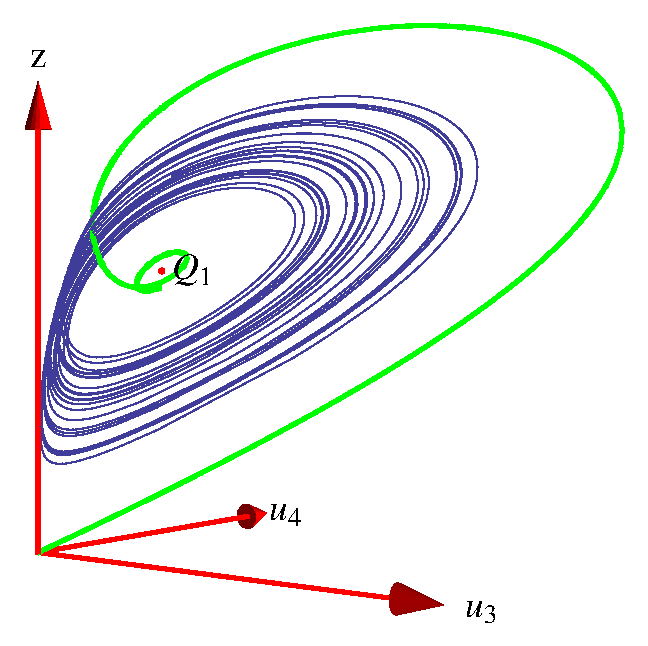
\includegraphics[width=.35\textwidth]{../../figs/CLEip1.eps} &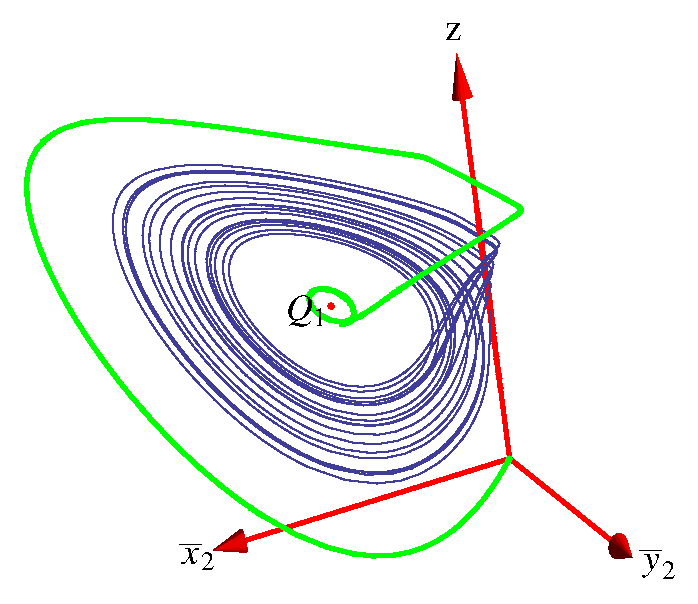
\includegraphics[width=.35\textwidth]{../../figs/CLEmfXYZ.eps} \\ 
		(\textit{a}) & (\textit{b}) 
	\end{tabular}
	\end{center}


\end{sheet}

	
\begin{sheet}{An efficient approach}


We need a method that can be implemented for \emph{high-dimensional} discretizations of PDE's
and it is sufficient for our purposes to be able to construct a \Poincare~section.
\begin{itemize}
 \item Do not attempt to rewrite the dynamics.
 \item Use geometric interpretation of moving frame method of Fels and Olver.
 \item Set up a group-invariant (as a set) \Poincare~section $\mathcal{P}_1$. Use
	a few of the first fundamental invariants that can be easily computed by
	the moving frame method. Here use $\overline{x}_2=\overline{y}_2$ or in original
	space $x_1^2+x_2^2=x_1 y_1 + x_2 y_2$.
 \item Think orbits as tori (generated by the action of the group)
 \item Since $\mathcal{P}_1$ is group-invariant it contains the group
	orbit of any point of intersection. 
 \item Set up a second section $\mathcal{P}_2$ that intersects each tori once. 
	Here use condition $\theta=0$ where $\theta$ the phase in complex $x$-plane. In practice instead of tracing the tori we apply the group transformation to set $\theta=0$ for points on $\mathcal{P}_1$.
 \item We only need to apply a linear transformation to map a point to $\mathcal{P}_2$ (globally
	the transformation is still non-linear and equivalent to \refeq{eq:mfinv}.)
\end{itemize}

 \begin{center}
 	 	\includegraphics[width=.35\textwidth]{../../figs/CLEmartiniPoster.eps}
 \end{center} 

\end{sheet}

 
\begin{sheet}{Return map}
 
 For CLE reduction through the use of the method proposed here allows the construction
 of a return map that accurately captures the dynamics
 \begin{center}
 	 	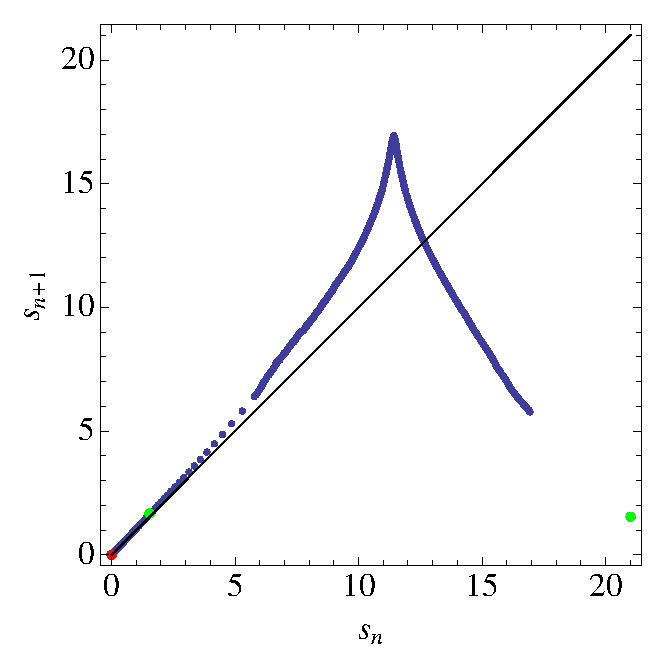
\includegraphics[width=.35\textwidth]{../../figs/CLEinvRM.eps}
 \end{center}
 Coordinate $s$ is Euclidean length along unstable manifold of \reqv~$Q_1$. 
 The map is approximatelly $1$-dimensional as a result of the very strong 
 contraction along the stable directions. The same map can be obtained through
 any reduction method.

 The map allows the determination of initial guesses for \rpo s of any given
 length that are then determined through multiple shooting to machine accuracy 
 in the original space.

\end{sheet}

\begin{sheet}{Future}
\begin{itemize}
 \item Test applicability to \KSe, \PCf.
 \item Use relative periodic orbits found in the framework of periodic orbit theory\cite{DasBuch} to compute asymptotic statistics of the attractor.
\end{itemize}


\end{sheet}


\begin{sheet}{References}
\begin{thebibliography}{99}
\bibitem{thisone}
	{\sc  E.~Siminos and P.~Cvitanovi\'c}, in preparation
\bibitem{DasBuch}
{\sc P.~Cvitanovi\'{c}, R.~Artuso, R.~Mainieri, G.~Tanner, and G.~Vattay}, {\em
  Chaos: Classical and Quantum}, Niels Bohr Institute, Copenhagen, 2005,
  ChaosBook.org.
\bibitem{cles}
{\sc A.C. Fowler, J.D. Gibbon and M.J. McGuinness}, 
    Physica D, 4, (1982), p.~139
\bibitem{NingHakenCLE90}
{\sc C. Ning and H. Haken},
    Physica D, 4, 1982, p. 139
\bibitem{FelsOlver98}
  {\sc M. Fels and P. J. Olver}, Acta Appl. Math., 1998, 51,
  p.~161
\bibitem{Gil07b}
  {\sc R. Gilmore and C. Letellier},
  \emph{The Symmetry of Chaos}, Oxford Univ. Press, 2007, Oxford
\bibitem{BakasovAbraham93}
    {\sc A.A. Bakasov and N.B. Abraham},
    Phys. Rev. A, 48, (1993), p.~1633


\end{thebibliography}
\end{sheet}



\end{poster}


\end{document}
